\documentclass[11pt]{article}

\usepackage[margin=1in]{geometry}
\usepackage{amsmath,amssymb}
\usepackage{booktabs}
\usepackage{graphicx}
\usepackage{natbib}
\usepackage{url}
\usepackage{hyperref}
\usepackage{setspace}
\onehalfspacing

\bibliographystyle{abbrvnat}
\setcitestyle{authoryear,round,citesep={;},aysep={,}}

\title{Quantifying the Inflation Tax (or Rebate) on Canadian Households}
\author{Working paper draft\\[0.5em]
\small Adaptation of \citep{wolff2023inflationtax}'s Methodology to Canada }
\date{\today}


\begin{document}
\maketitle

% Editable short abstract (source of truth for revision): docs/abstract.md
% Extended abstract: docs/extended_abstract.md
\begin{abstract}
 \citep{wolff2023inflationtax} introduced the net inflation gain identity $NIG=IG-IT$, matching the well-known negative effect of inflation on income (`tax' = $IT$) against balance-sheet gains from debt devaluation and asset revaluation (=$IG$). Intuitively, things get more expensive, but your balance sheet may improve to mitigate this - or worsen it - depending on your different exposures.
 
 This paper brings this accounting framework to Canada, to account for the relative impact of inflation on different households, using the Survey of Financial Security (SFS, 1999--2023). We construct equivalent metrics for marketable net worth and portfolios, compute net inflation gains ($NIG$) by wealth quintile, tenure, age, and region. Middle Canadian wealth quintiles typically record positive $NIG$ relative to income, qualitatively echoing Wolff's U.S.\ conclusion that inflation is ``not a tax'' for the middle class, but instead something of a rebate. Meanwhile the bottom quintile is more exposed to the income tax $IT$ deteriorating their earnings, due to small wealth holdings giving little opportunities to gain from nominal appreciation. While the SFS is not designed to represent the ultra-wealthy, we do find that the wealth benefit the most, due to high equity and business holdings. Leverage and debt deflation does not have an appreciable effect for this group, but is instead much more present for the middle classes. This pattern is not constant over time, with 2016-2019 offering a time when $NIG$ is negative, instead of the usual positive, for the richer groups. Tenure patterns show strong differences, with renters showing the lowest $NIG$ relative to income. However, the results diverge from a pure leverage narrative: free-and-clear owners show higher $NIG$/income than mortgagors, likely due to larger equity holdings and higher wealth generally.
\end{abstract}

\section{Introduction}

Public debate on inflation emphasizes real-income erosion. \citet{wolff2023inflationtax} argues that this ``inflation tax'' on income must be paired with balance-sheet gains: inflation reduces the real burden of nominal debt and can raise the present value of claims discounted at real interest rates. The net inflation gain ($NIG$) can therefore be positive for leveraged middle-class households even when real incomes are squeezed.

Figure~\ref{fig:macro_context} places the Canadian episode in a longer macro backdrop from the late 1990s to the present. The Bank of Canada's target overnight rate fell from the mid--single digits into a long low-rate stretch after the global financial crisis, then rose sharply in 2022--23 as CPI inflation peaked near 7~percent. Over the same window, residential property prices (BIS Canada index) and the S\&P/TSX Composite delivered large positive---and occasionally sharply negative---annual returns, while nominal SEPH earnings growth was typically in the 2--4~percent range outside the pandemic spike. Vertical dashed lines mark Survey of Financial Security (SFS) waves (1999, 2005, 2012, 2016, 2019, 2023): the balance-sheet accounting below is observed only at those dates, against this continuous rate, inflation, and asset-price path.

\begin{figure}[ht]
\centering
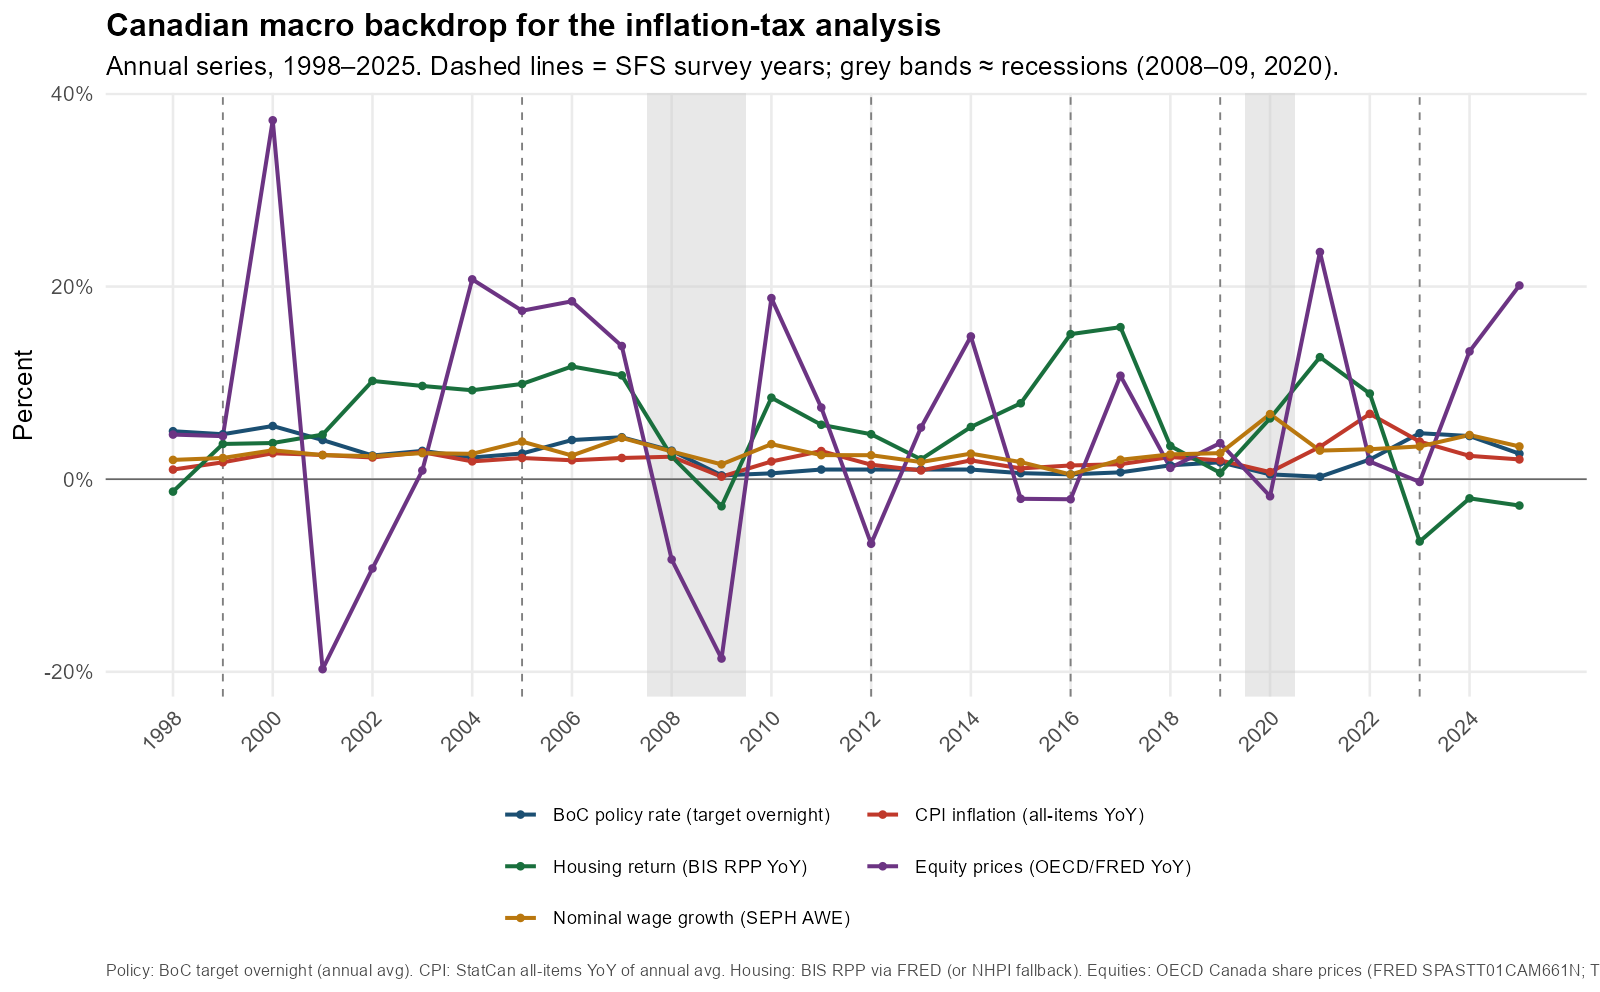
\includegraphics[width=0.95\textwidth]{../output/figures/macro_context_1998_present.png}
\caption{Canadian macro context, approximately 1998 to present: Bank of Canada target overnight rate (annual average), all-items CPI inflation, residential property-price appreciation (BIS), Canadian equity-price returns (S\&P/TSX when available; otherwise OECD share prices via FRED), and nominal average weekly earnings growth. Dashed lines mark SFS survey years; grey bands approximate recessions (2008--09, 2020). Sources and series definitions are documented in the repository (\texttt{data/external/MACRO\_CONTEXT\_SOURCES.md}).}
\label{fig:macro_context}
\end{figure}

This draft implements that accounting for Canada. The empirical engine lives in the accompanying repository and reads the Canadian Survey of Financial Security (SFS) rather than the U.S.\ Survey of Consumer Finances (SCF).

\section{Related literature}
\label{sec:lit}
% Annotated literature note with URLs/DOIs: docs/06_literature_review.md

A large literature measures how wealth is distributed and how asset prices and interest rates reshape that distribution. Using historical Survey of Consumer Finances (SCF) microdata, \citet{kuhn2020inequality} show that middle-class portfolios are housing-intensive while rich households hold business equity, so differential asset-price paths drive U.S.\ wealth inequality even when income inequality moves differently. Federal Reserve work on the SCF and the Distributional Financial Accounts provides the modern infrastructure for these facts: \citet{bricker2016measuring} reconcile survey and administrative top shares, and \citet{batty2019dfa,batty2022dfa} construct quarterly DFA wealth distributions consistent with the Financial Accounts. Related asset-pricing research links equity returns and low required returns to movements in top wealth shares and to welfare redistribution that depends on net sales rather than holdings alone \citep{gomez2025assetprices,gomez2024lowrate,fagereng2025apr}. For Canada, \citet{hempel2025wealth} capitalizes incomes to estimate a top 1\% wealth share that peaked near 21\% before the Global Financial Crisis and stood near 19\% in 2022---below U.S.\ levels---while the Parliamentary Budget Officer's High-net-worth Families Database implies a still higher corrected top share \citep{dong2025toptail}, and Statistics Canada's Distributions of Household Economic Accounts align the Survey of Financial Security with national balance-sheet totals \citep{statcan2025dhea}.

Against this measurement backdrop, a complementary literature treats inflation as a redistributive balance-sheet event. \citet{doepke2006inflation} document large net nominal positions and show that surprise inflation transfers wealth from old bondholders toward young middle-class debtors. \citet{auclert2019redistribution} embeds Fisher, interest-rate exposure, and earnings-heterogeneity channels in the transmission of monetary policy when marginal propensities to consume covary with exposures. \citet{wolff2021inflation,wolff2023inflationtax} operationalize related ideas in transparent SCF accounting identities. Defining an inflation tax on income and an inflation gain on assets and debts, Wolff constructs the net inflation gain $NIG=IG-IT$ and finds that U.S.\ middle wealth quintiles---and, under his assumptions, the ultra-wealthy---often record large positive $NIG$ relative to income, while bottom quintiles are hurt; related interest-rate and inflation revaluations also reduced measured wealth inequality over 1983--2019 even as overall inequality rose for other reasons. These $NIG$ metrics are useful precisely because they force income-side ``inflation tax'' rhetoric to confront leverage, liquid-asset losses, and duration-sensitive revaluation of equities, businesses, and bonds.

Canada's policy debate places special weight on housing affordability and household cash-flow stress, so the relative roles of inflation, interest rates, tenure, and geography are first-order. Canadian mortgages typically renew on short fixed terms, so rate cycles transmit to payments more quickly than under U.S.\ 30-year fixed-rate contracts; Bank of Canada staff work finds material and persistent consumption effects of the recent hike cycle on mortgagors \citep{bouras2024mortgage}. This paper adapts Wolff's $NIG$ framework to the Canadian Survey of Financial Security. Because the SFS lacks an SCF-style high-income oversample, we emphasize wealth quintiles and tenure rather than ultra-top cells, using \citet{hempel2025wealth} and PBO estimates only to bound top-tail understatement. The Canadian application is informative both where it echoes Wolff---positive middle-quintile $NIG$/income in many episodes---and where institutions differ, including free-and-clear versus mortgagor patterns and periods of rising real yields.

\section{Methodology}

\subsection{Definitions \citep{wolff2023inflationtax}}

Let $INF$ denote CPI inflation, $INC$ household income, $LIQ$ liquid assets, and $DBT$ debt. Stocks, business equity, and bonds are revalued using a Fisher wedge between nominal and real discount rates (with floors to avoid explosive $1/r$ terms in the low-rate Canadian sample). Then
\begin{align}
IG &= \Delta STK + \Delta BUS + \Delta BND - LIQ\cdot INF + DBT\cdot INF,\\
IT &= INC\cdot INF,\\
NIG &= IG - IT.
\end{align}
Wealth is marketable net worth excluding vehicles and defined-benefit pension wealth. Non-registered mutual funds are allocated 60 percent equity and 40 percent bonds. Because the SFS reports registered-account \emph{totals} without asset-class detail, we follow the Parliamentary Budget Officer's TFSA methodology and set each household's RRSP/RRIF/TFSA look-through mix equal to its non-registered financial mix in the SFS.\footnote{\citet{pbo2015tfsa}: ``TFSA portfolio composition is assumed to be identical to those observed in non-registered investment accounts of the Survey of Financial Security.'' We apply the same rule to RRSP, RRIF, and other retirement balances. Tax-efficient asset location implies this likely \emph{understates} the equity share inside registered plans---especially TFSAs---so stock-channel inflation gains are conservative on that margin.}

\subsection{Interest rates and inequality \citep{wolff2021inflation}}

Between SFS waves we hold start-of-period portfolios fixed and attribute wealth changes to movements in real GoC 10-year yields, bond duration effects, cumulative inflation on liquid assets and debt, and (separately) a Canadian mortgage-affordability house-price factor based on five-year terms and 25-year amortizations.

\subsection{Data}

SFS economic-family PUMF waves: 1999, 2005, 2012, 2016, 2019, 2023. Macro inputs: Statistics Canada CPI; Bank of Canada 10-year yields; conventional five-year mortgage rates. Survey weights ($pweight$) are used throughout.

\section{Preliminary Canadian results}

Figure~\ref{fig:nig2023} reports $NIG$ as a share of mean income by wealth quintile in 2023. Middle quintiles show substantial positive ratios; the bottom quintile is near zero; the top quintile's large ratio is sensitive to equity holdings and discount-rate assumptions and should be interpreted cautiously given PUMF top-coding.

\begin{figure}[ht]
\centering
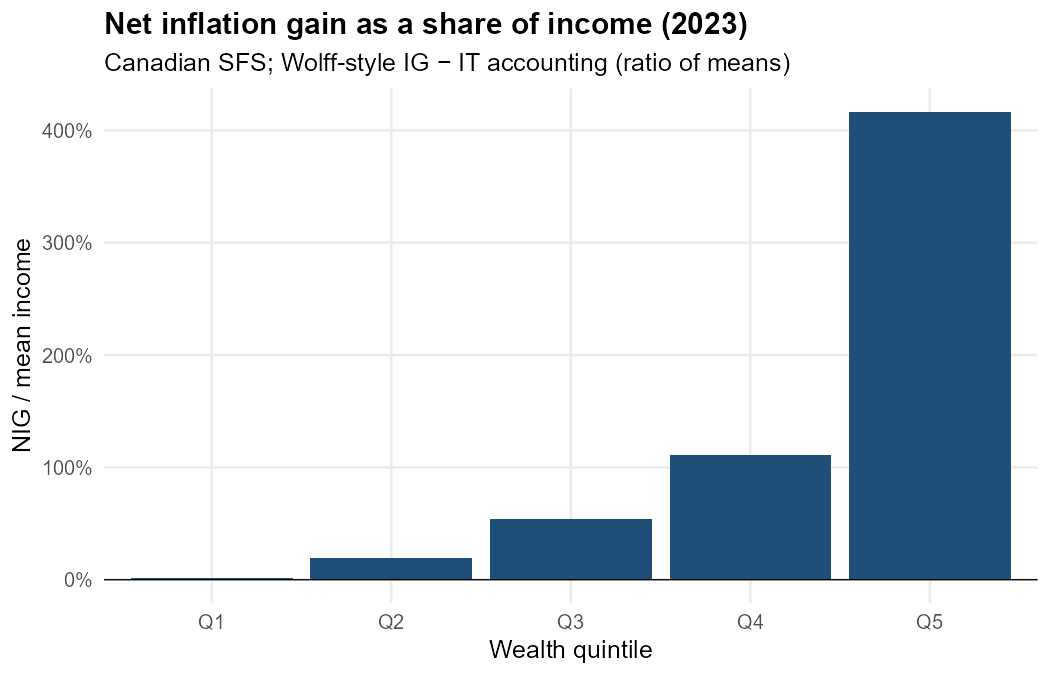
\includegraphics[width=0.85\textwidth]{../output/figures/nig_pct_income_latest.png}
\caption{Net inflation gain over mean income by wealth quintile, SFS 2023.}
\label{fig:nig2023}
\end{figure}

\subsection{Composition of top-quintile gains}

Large $NIG$ (and large losses) in the top wealth quintile are driven primarily by long-duration equity and business revaluation, not by leverage. In 2023, mean stock plus business holdings are on the order of \$900{,}000 in Q5 versus about \$30{,}000 in Q3, and the stock and business terms together account for roughly 85\% of Q5 inflation gain ($IG$). Debt-to-asset ratios are lowest at the top (about 0.08 versus 0.28 in Q3), so debt devaluation is only a small share of $IG$ for Q5, and the income tax ($IT$) barely offsets those asset-side gains. Middle and lower quintiles rely relatively more on the debt-devaluation channel. The 2016--2019 episode---when real yields rose---flips the sign of the same equity/business channel, producing large Q5 losses. Magnitudes remain fragile given PUMF top-coding and the absence of a high-income oversample.

Period decompositions (Figure~\ref{fig:period}) show that episodes of falling real yields (e.g.\ 2005--2012) amplify asset-side gains, while 2016--2019---when real yields rose---produces negative net gains for several classes despite positive debt devaluation.

We retain Wolff's 30-year FRM affordability schedule as a benchmark and present Canadian 25-/30-year amortization schedules alongside. Results are also split by owners with mortgages, free-and-clear owners, and renters. We do \emph{not} evaluate the distribution of homeowner risk arising from short Canadian contract terms; detailed interest-rate pass-through is deferred.

\begin{figure}[ht]
\centering
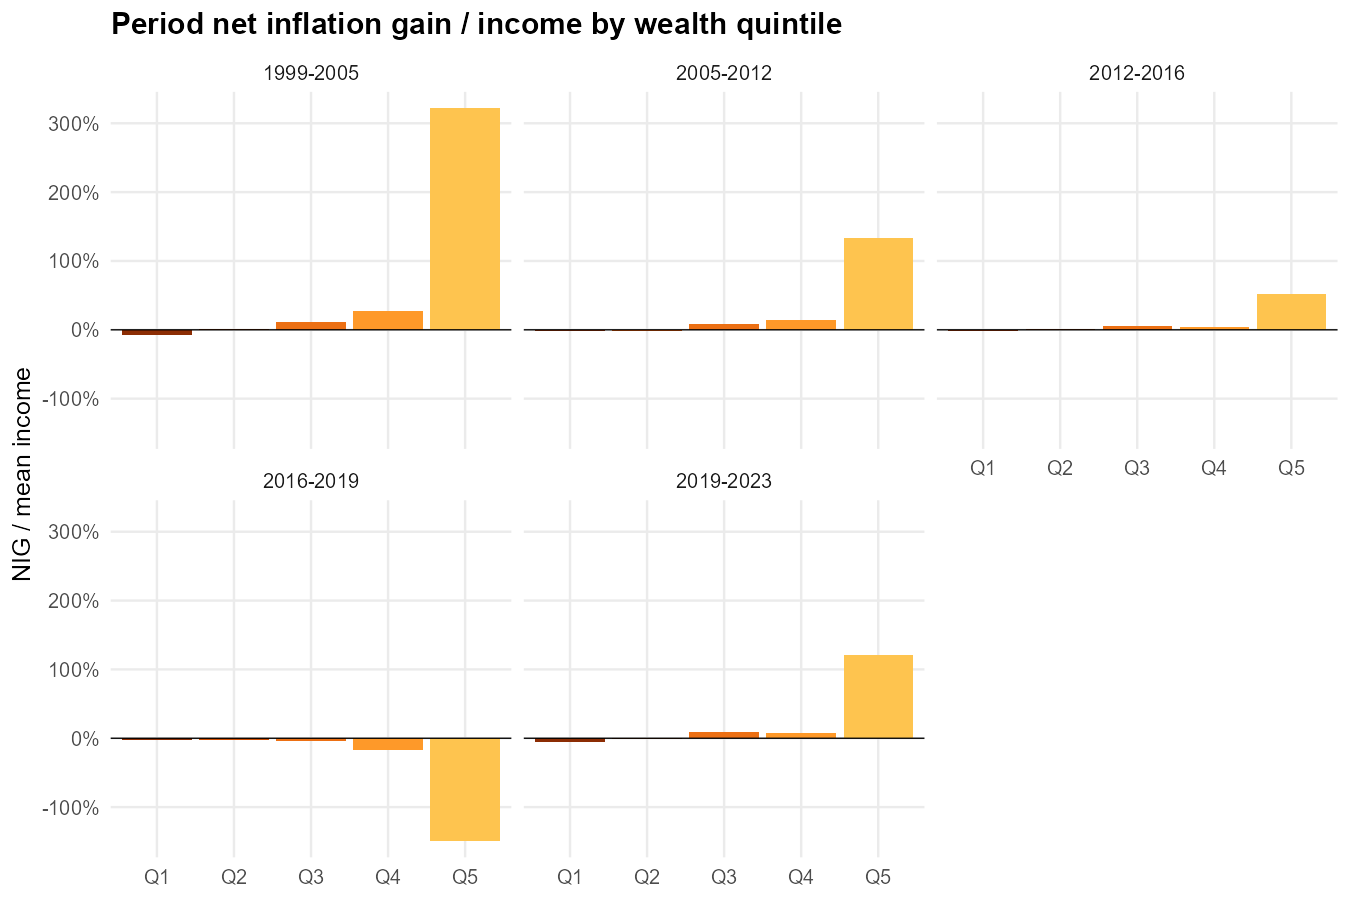
\includegraphics[width=0.95\textwidth]{../output/figures/nig_period_by_quintile.png}
\caption{Period $NIG$/income by wealth quintile.}
\label{fig:period}
\end{figure}

\section{Interest rates and the household balance sheet}
% Plan and checklist: docs/07_interest_rate_section_plan.md
% Scope: Wolff WP 29392-style direct revaluation (real GoC yields, bond duration,
% inflation on liquid assets/debt, optional mortgage-affordability housing).
% Core NIG (above) continues to exclude the housing affordability term (WP 31775).

% TODO: Summarize Wolff's channels (STK/BUS real-rate PV; bonds; nominal-mortgage
%       housing affordability; LIQ/DBT inflation) and explicit exclusions
%       (mortgage cash-flow as expenditure not NW; indirect GE effects).
% TODO: Table --- period mean/median/Gini actual vs revalued (no housing / CA 25y /
%       Wolff 30y amort); contribution shares of mean (median) change by channel.
% TODO: Figure --- stacked channel contributions; Gini path actual vs counterfactual.
% TODO: Canadian adaptations --- 5y conventional rates, 25y/30y amort, duration
%       fallback at low real rates, SFS waves 1999--2023; tenure and age incidence.
% TODO: Restate deferrals --- renewal-risk incidence and detailed pass-through remain
%       out of scope; still deliver relative-role accounting and coded sensitivities
%       (3y-rate proxy, stress rate). See docs/07_interest_rate_section_plan.md.

\section{Barriers and limitations}

Key barriers relative to Wolff's SCF setting include: (i) only six survey years; (ii) no SCF-style high-income oversample; (iii) incomplete race/ethnicity measures on the PUMF; (iv) need to impute equity/bond splits inside registered accounts; (v) Canadian fixed-term mortgages rather than U.S.\ 30-year FRMs. Core $NIG$ remains SFS-only. As an additional contribution we append a recent-window consumption lens from the Survey of Household Spending (2017--2023 only): necessities and shelter shares of current consumption by income quintile, tenure, and analytic region, with income$\times$tenure proxies in place of wealth quintiles (unavailable on SHS). SHS and SFS units differ (household vs.\ economic family) and the post-2010 SHS redesign precludes splicing to the full SFS history.

\subsection{Measurement of the top of the wealth distribution}

Unlike the U.S.\ Survey of Consumer Finances, the Canadian Survey of Financial Security lacks a high-income list sample and, on the public-use file, is subject to top-coding. As a result, this paper cannot speak reliably about the ultra-wealthy in the sense of Wolff's SCF analyses. Independent work that corrects for under-coverage at the extreme upper tail confirms that raw SFS top shares are too low, while also placing Canadian concentration well below U.S.\ levels. Using the income capitalization method, \citet{hempel2025wealth} estimates a top 1\% wealth share of about 19.3\% in 2022---roughly three to five percentage points above unadjusted SFS figures---along a path from 16.2\% in 1990 to a peak of 21.3\% in 2008 and then roughly 17.5--19.3\% through 2022. The cumulative rise of 3.1 percentage points over 1990--2022 is less than half the increase observed in the United States and France over a similar period, and the Canadian level remains substantially below U.S.\ estimates in the neighbourhood of 30--37\%.\footnote{U.S.\ comparisons draw on \citet{saezzucman2016} and \citet{batty2022dfa} as reported in \citet{hempel2025wealth}.} The Parliamentary Budget Officer's 2025 High-net-worth Families Database (HFD), which combines the SFS with Pareto interpolation and rich lists, implies an even larger correction at the very top: a 2023 top 1\% share of 23.8\% versus 11.0\% in the SFS alone.\footnote{\citet{dong2025toptail}. The SFS--HFD gap narrows sharply below the 80th percentile; the SFS is designed to support representative net-worth estimates roughly up to the top 5\% of the distribution.} \citeauthor{hempel2025wealth}'s capitalization series lies between raw SFS and PBO HFD levels; the remaining discrepancy with the Pareto-based HFD is concentrated in the top 0.1\% \citep{hempel2025wealth}.

For the inflation-tax accounting in this paper, these findings have a clear implication. We prefer cuts that the SFS can support---wealth quintiles and, where a finer upper cut is useful, the P80--90 band---rather than P99 or other ultra-top cells. The top quintile (Q5) remains fragile for interpretation of large $NIG$/income ratios. We do not reweight or append synthetic top-tail observations to the SFS PUMF; external Hempel and PBO estimates are used only to bound inference. More importantly for net inflation gain ($NIG$), Canadian wealth concentration has not risen in the U.S.\ manner over recent decades, so any equity- or business-revaluation channel concentrated at the top is operating against a more muted concentration backdrop than in Wolff's U.S.\ setting.

\section{Next steps}

Refine registered-account allocation sensitivities; add bootstrap inference for 2023; report P80--90 rather than P99 as the preferred ``upper middle / affluent'' cut; integrate SHS consumption figures into the paper body or appendix; and complete the full working-paper text.

\bibliography{references}

\end{document}
